

\actTitle{Worksheet 3.3}


\noindent \textbf{Instructions:} Work together in groups of 3 or 4 to
complete the following problems.

Student goals:
  \begin{itemize}
  \item Use the logarithm function to solve for a variable in an
    equation that has exponential terms.
  \item Determine the domain and range of a simple function that
    contains logarithmic terms.
  \item Determine the inverse of a simple exponential function.
  \item Determine the inverse of a function that contains logarithmic terms.
  \item Graph basic logarithmic functions.
  \item Solve for a variable in a simple equation that contains logarithmic
    terms.
  %\item Recognize that $\log(x)=\log_{10}(x)$.
  %\item Recognize that $\ln(x)=\log_e(x)$.
  \end{itemize}



\begin{enumerate}
\item Write each of the following functions in their equivalent  exponential forms.
  $$\log_3(x)=9,   \quad \quad \quad \quad
  \log_2(8)=x,     \quad \quad \quad \quad
  \log_2(y)=5,     \quad \quad  \quad \quad
  \log_5(y)=2.$$
\vfill
\item Write each of the following functions in their equivalent  logarithmic forms.
  $$y=3^4,  \quad \quad \quad \quad \quad \quad
  m=4^2,    \quad \quad \quad \quad \quad \quad
  64=4^x,   \quad \quad \quad \quad  \quad \quad
  32=x^5.$$
\vfill
\item Solve each of the following expressions for the unknown value by
  first rewriting the equation in exponential form.
\begin{enumerate}
\item $\log_3(x)=4$
\vfill
\vfill
\item $\log_{m}(81)=4$
\vfill
\vfill
\item $\displaystyle \log_2\left(\frac{x}{2}\right)=5$
\vfill
\vfill
\item $\log_2(4x)=5$
\vfill
\vfill
\end{enumerate}



\clearpage
\item Determine the inverse of each of the following functions.
  (Hint: rewrite each expression in logarithmic or exponential form
  after switching $x$ and $y$.)  Determine the domain and range of the
  function and its inverse.
\begin{enumerate}
\item $f(x)=\log_3(x)$, \quad \quad \quad $f^{-1}(x)=$
\begin{flushright}
 Domain of $f(x)$:  \quad \quad \quad\quad\quad\quad Range of $f(x)$:\quad\quad\quad\quad \vfill
Domain of $f^{-1}(x)$:   \quad \quad\quad\quad\quad Range of $f^{-1}(x)$:\quad\quad\quad\quad
\end{flushright}
\vfill
\item $g(x)=\log_5(x+3)$,  \quad \quad \quad $g^{-1}(x)=$
\begin{flushright}
Domain of $g(x)$:  \quad \quad \quad\quad\quad\quad Range of $g(x)$:\quad\quad\quad\quad \vfill
Domain of $g^{-1}(x)$:   \quad \quad\quad\quad\quad Range of $g^{-1}(x)$:\quad\quad\quad\quad
\end{flushright}

\vfill 
\item $h(x)=\ln(7x-4)$,  \quad \quad \quad $h^{-1}(x)=$
\begin{flushright}
Domain of $h(x)$:  \quad \quad \quad\quad\quad\quad Range of $h(x)$:\quad\quad\quad\quad \vfill 
Domain of $h^{-1}(x)$:   \quad \quad\quad\quad\quad Range of $h^{-1}(x)$:\quad\quad\quad\quad
\end{flushright}

\clearpage

\vfill
\item $\displaystyle k(x)=4^{x+3}$  \quad \quad \quad $k^{-1}(x)=$
\begin{flushright}
Domain of $k(x)$:  \quad \quad \quad\quad\quad\quad Range of $k(x)$:\quad\quad\quad\quad \vfill
Domain of $k^{-1}(x)$:   \quad \quad\quad\quad\quad  Range of $k^{-1}(x)$:\quad\quad\quad\quad
\end{flushright}

\vfill
\item $p(x)=e^{3x}$  \quad \quad \quad $p^{-1}(x)=$
\begin{flushright}
Domain of $p(x)$:  \quad \quad \quad\quad\quad\quad Range of $p(x)$:\quad\quad\quad\quad \vfill 
Domain of $p^{-1}(x)$:   \quad \quad\quad\quad\quad Range of $p^{-1}(x)$:\quad\quad\quad\quad
\end{flushright}

\vfill
\end{enumerate}
  
\item Graph $q(x)=2^x$ and $q^{-1}(x)=\log_2(x)$ on the rectangular
  coordiantes below. Also, graph and label their asymptotes.

\begin{itemize}
\begin{multicols}{2}
\item[(a)] $q(x)=2^x$

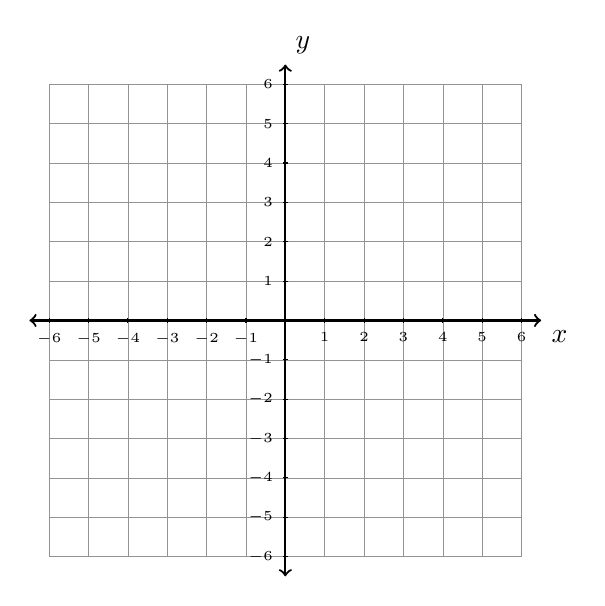
\begin{tikzpicture}[y=.5cm, x=.5cm,font=\sffamily,
	mydot/.style={
    circle,
    fill=white,
    draw,
    outer sep=0pt,
    inner sep=1.5pt
  }]
    %% Add a grid
    \draw[step = 1, gray, very thin,opacity=0.85] (-6, -6) grid (6, 6);
 	%% Draw the axes
	\draw[thick,<->] (-6.5,0) -- coordinate (x axis mid) (6.5,0) node[anchor = north west] {$x$};
    \draw[thick,<->] (0,-6.5) -- coordinate (y axis mid) (0,6.5) node[anchor = south west] {$y$};
    %% Label the y axis
    \foreach \y in {-6,...,-1,1,2,...,6} {
      \draw (1pt, \y) -- (-1pt, \y) node[anchor =  east] {\tiny$\y$};
    }
    %% Label the x axis
    \foreach \x in {-6,...,-1,1,2,...,6} {
      \draw (\x,1pt) -- (\x,-1pt) node[anchor = north] {\tiny$\x$};
    }
    %% Draw the function.
 %   \begin{scope}
 %        \draw[very thick,black] (-3,2) -- (1,1);
 %        \draw[very thick,black] (3.05,1.05) -- (4,3);
    %semi-circle
  %       \draw[very thick, black] (1,1) arc [radius=1, start angle=180, end angle= 5];
     %parabola
     %    \draw[ultra thick, black, domain=-5:0] plot (\x, {(-0.2)*(\x-5)*(\x+5)});
     %dots
     %  \fill[black] (-3, 2) circle[radius=0.5ex];
     %   \fill[black] (1,1) circle[radius=0.5ex];
     %    \fill[black] (4,3) circle[radius=0.5ex];
     %     \draw[very thick, black] (3,1) circle[radius=0.5ex];


   % \end{scope}

    %%\node[above=0.1cm] at (-2,2 )   {\nextXValue};

  \end{tikzpicture}

\vspace{1in}


\item[(b)] $q^{-1}(x)=\log_2(x)$ 

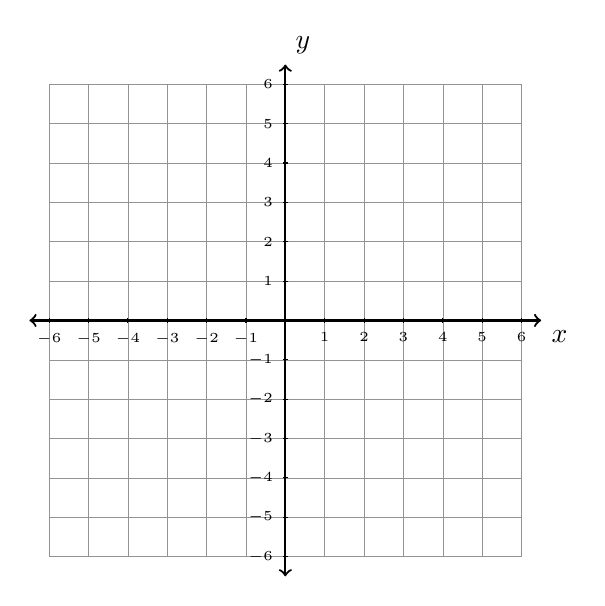
\begin{tikzpicture}[y=.5cm, x=.5cm,font=\sffamily,
	mydot/.style={
    circle,
    fill=white,
    draw,
    outer sep=0pt,
    inner sep=1.5pt
  }]
    %% Add a grid
    \draw[step = 1, gray, very thin,opacity=0.85] (-6, -6) grid (6, 6);
 	%% Draw the axes
	\draw[thick,<->] (-6.5,0) -- coordinate (x axis mid) (6.5,0) node[anchor = north west] {$x$};
    \draw[thick,<->] (0,-6.5) -- coordinate (y axis mid) (0,6.5) node[anchor = south west] {$y$};
    %% Label the y axis
    \foreach \y in {-6,...,-1,1,2,...,6} {
      \draw (1pt, \y) -- (-1pt, \y) node[anchor =  east] {\tiny$\y$};
    }
    %% Label the x axis
    \foreach \x in {-6,...,-1,1,2,...,6} {
      \draw (\x,1pt) -- (\x,-1pt) node[anchor = north] {\tiny$\x$};
    }
    %% Draw the function.
 %   \begin{scope}
 %        \draw[very thick,black] (-3,2) -- (1,1);
 %        \draw[very thick,black] (3.05,1.05) -- (4,3);
    %semi-circle
  %       \draw[very thick, black] (1,1) arc [radius=1, start angle=180, end angle= 5];
     %parabola
     %    \draw[ultra thick, black, domain=-5:0] plot (\x, {(-0.2)*(\x-5)*(\x+5)});
     %dots
     %  \fill[black] (-3, 2) circle[radius=0.5ex];
     %   \fill[black] (1,1) circle[radius=0.5ex];
     %    \fill[black] (4,3) circle[radius=0.5ex];
     %     \draw[very thick, black] (3,1) circle[radius=0.5ex];


   % \end{scope}

    %%\node[above=0.1cm] at (-2,2 )   {\nextXValue};

  \end{tikzpicture}


\end{multicols}
\end{itemize}

\vfill


\clearpage


\item Graph each of the following transformed logarithmic functions.  

\begin{itemize}

\item[(a)] $m(x)=\log_2(-x+3)+1$

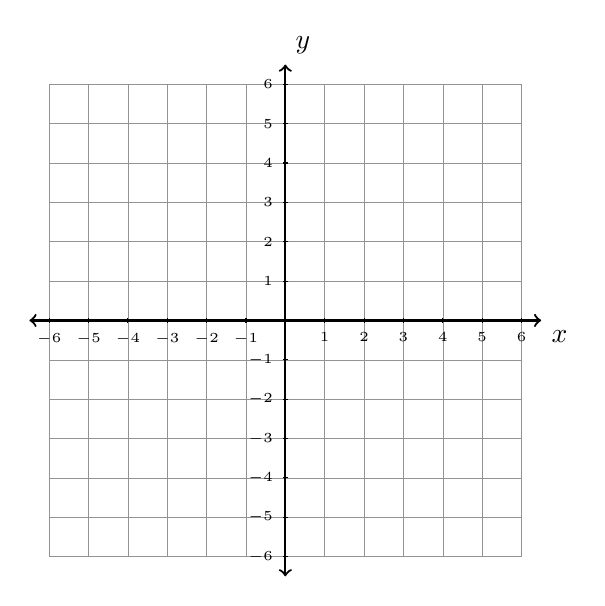
\begin{tikzpicture}[y=.5cm, x=.5cm,font=\sffamily,
	mydot/.style={
    circle,
    fill=white,
    draw,
    outer sep=0pt,
    inner sep=1.5pt
  }]
    %% Add a grid
    \draw[step = 1, gray, very thin,opacity=0.85] (-6, -6) grid (6, 6);
 	%% Draw the axes
	\draw[thick,<->] (-6.5,0) -- coordinate (x axis mid) (6.5,0) node[anchor = north west] {$x$};
    \draw[thick,<->] (0,-6.5) -- coordinate (y axis mid) (0,6.5) node[anchor = south west] {$y$};
    %% Label the y axis
    \foreach \y in {-6,...,-1,1,2,...,6} {
      \draw (1pt, \y) -- (-1pt, \y) node[anchor =  east] {\tiny$\y$};
    }
    %% Label the x axis
    \foreach \x in {-6,...,-1,1,2,...,6} {
      \draw (\x,1pt) -- (\x,-1pt) node[anchor = north] {\tiny$\x$};
    }
    %% Draw the function.
 %   \begin{scope}
 %        \draw[very thick,black] (-3,2) -- (1,1);
 %        \draw[very thick,black] (3.05,1.05) -- (4,3);
    %semi-circle
  %       \draw[very thick, black] (1,1) arc [radius=1, start angle=180, end angle= 5];
     %parabola
     %    \draw[ultra thick, black, domain=-5:0] plot (\x, {(-0.2)*(\x-5)*(\x+5)});
     %dots
     %  \fill[black] (-3, 2) circle[radius=0.5ex];
     %   \fill[black] (1,1) circle[radius=0.5ex];
     %    \fill[black] (4,3) circle[radius=0.5ex];
     %     \draw[very thick, black] (3,1) circle[radius=0.5ex];


   % \end{scope}

    %%\node[above=0.1cm] at (-2,2 )   {\nextXValue};

  \end{tikzpicture}

\vspace{1in}


\item[(b)] $w^{-1}(x)=2\log_3(x+4)-1$ 

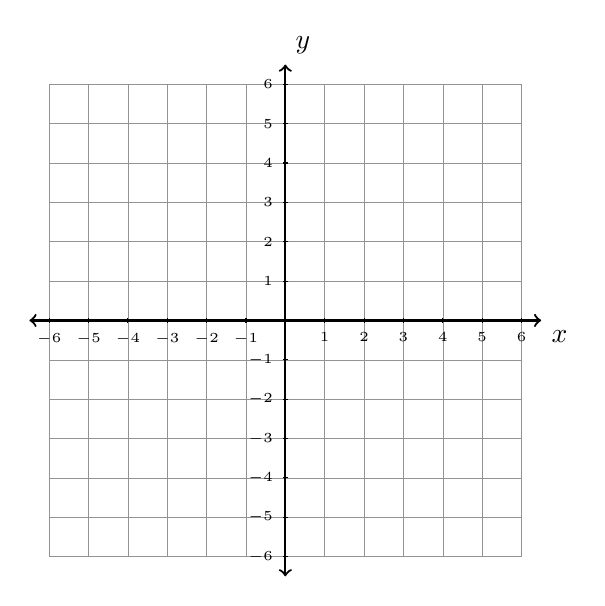
\begin{tikzpicture}[y=.5cm, x=.5cm,font=\sffamily,
	mydot/.style={
    circle,
    fill=white,
    draw,
    outer sep=0pt,
    inner sep=1.5pt
  }]
    %% Add a grid
    \draw[step = 1, gray, very thin,opacity=0.85] (-6, -6) grid (6, 6);
 	%% Draw the axes
	\draw[thick,<->] (-6.5,0) -- coordinate (x axis mid) (6.5,0) node[anchor = north west] {$x$};
    \draw[thick,<->] (0,-6.5) -- coordinate (y axis mid) (0,6.5) node[anchor = south west] {$y$};
    %% Label the y axis
    \foreach \y in {-6,...,-1,1,2,...,6} {
      \draw (1pt, \y) -- (-1pt, \y) node[anchor =  east] {\tiny$\y$};
    }
    %% Label the x axis
    \foreach \x in {-6,...,-1,1,2,...,6} {
      \draw (\x,1pt) -- (\x,-1pt) node[anchor = north] {\tiny$\x$};
    }
    %% Draw the function.
 %   \begin{scope}
 %        \draw[very thick,black] (-3,2) -- (1,1);
 %        \draw[very thick,black] (3.05,1.05) -- (4,3);
    %semi-circle
  %       \draw[very thick, black] (1,1) arc [radius=1, start angle=180, end angle= 5];
     %parabola
     %    \draw[ultra thick, black, domain=-5:0] plot (\x, {(-0.2)*(\x-5)*(\x+5)});
     %dots
     %  \fill[black] (-3, 2) circle[radius=0.5ex];
     %   \fill[black] (1,1) circle[radius=0.5ex];
     %    \fill[black] (4,3) circle[radius=0.5ex];
     %     \draw[very thick, black] (3,1) circle[radius=0.5ex];


   % \end{scope}

    %%\node[above=0.1cm] at (-2,2 )   {\nextXValue};

  \end{tikzpicture}
  \clearpage

\item[(c)] $u(x)=-3\ln(x-2)$

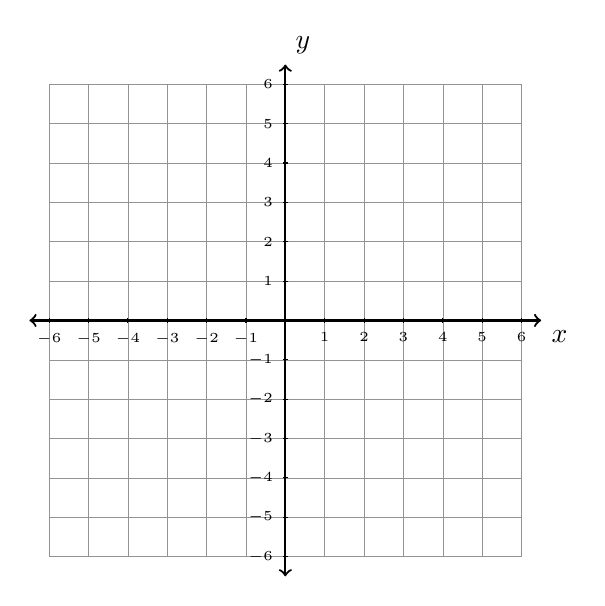
\begin{tikzpicture}[y=.5cm, x=.5cm,font=\sffamily,
	mydot/.style={
    circle,
    fill=white,
    draw,
    outer sep=0pt,
    inner sep=1.5pt
  }]
    %% Add a grid
    \draw[step = 1, gray, very thin,opacity=0.85] (-6, -6) grid (6, 6);
 	%% Draw the axes
	\draw[thick,<->] (-6.5,0) -- coordinate (x axis mid) (6.5,0) node[anchor = north west] {$x$};
    \draw[thick,<->] (0,-6.5) -- coordinate (y axis mid) (0,6.5) node[anchor = south west] {$y$};
    %% Label the y axis
    \foreach \y in {-6,...,-1,1,2,...,6} {
      \draw (1pt, \y) -- (-1pt, \y) node[anchor =  east] {\tiny$\y$};
    }
    %% Label the x axis
    \foreach \x in {-6,...,-1,1,2,...,6} {
      \draw (\x,1pt) -- (\x,-1pt) node[anchor = north] {\tiny$\x$};
    }
    %% Draw the function.
 %   \begin{scope}
 %        \draw[very thick,black] (-3,2) -- (1,1);
 %        \draw[very thick,black] (3.05,1.05) -- (4,3);
    %semi-circle
  %       \draw[very thick, black] (1,1) arc [radius=1, start angle=180, end angle= 5];
     %parabola
     %    \draw[ultra thick, black, domain=-5:0] plot (\x, {(-0.2)*(\x-5)*(\x+5)});
     %dots
     %  \fill[black] (-3, 2) circle[radius=0.5ex];
     %   \fill[black] (1,1) circle[radius=0.5ex];
     %    \fill[black] (4,3) circle[radius=0.5ex];
     %     \draw[very thick, black] (3,1) circle[radius=0.5ex];


   % \end{scope}

    %%\node[above=0.1cm] at (-2,2 )   {\nextXValue};

  \end{tikzpicture}

\vspace{1in}


\item[(d)] $v^{-1}(x)=\log_5(5-x)$ 

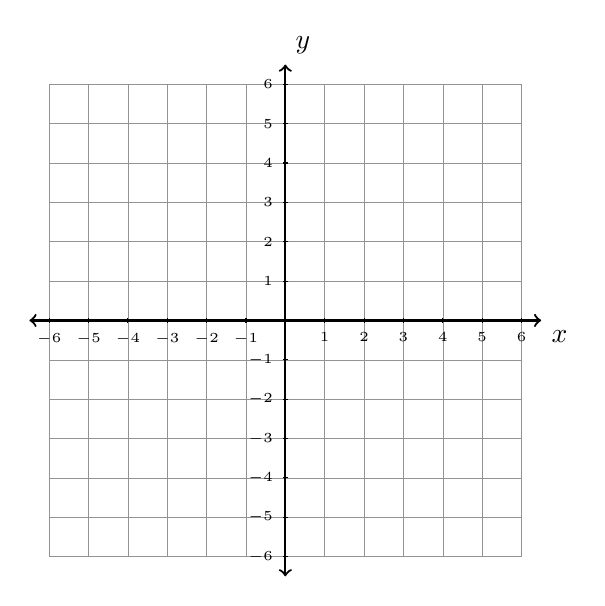
\begin{tikzpicture}[y=.5cm, x=.5cm,font=\sffamily,
	mydot/.style={
    circle,
    fill=white,
    draw,
    outer sep=0pt,
    inner sep=1.5pt
  }]
    %% Add a grid
    \draw[step = 1, gray, very thin,opacity=0.85] (-6, -6) grid (6, 6);
 	%% Draw the axes
	\draw[thick,<->] (-6.5,0) -- coordinate (x axis mid) (6.5,0) node[anchor = north west] {$x$};
    \draw[thick,<->] (0,-6.5) -- coordinate (y axis mid) (0,6.5) node[anchor = south west] {$y$};
    %% Label the y axis
    \foreach \y in {-6,...,-1,1,2,...,6} {
      \draw (1pt, \y) -- (-1pt, \y) node[anchor =  east] {\tiny$\y$};
    }
    %% Label the x axis
    \foreach \x in {-6,...,-1,1,2,...,6} {
      \draw (\x,1pt) -- (\x,-1pt) node[anchor = north] {\tiny$\x$};
    }
    %% Draw the function.
 %   \begin{scope}
 %        \draw[very thick,black] (-3,2) -- (1,1);
 %        \draw[very thick,black] (3.05,1.05) -- (4,3);
    %semi-circle
  %       \draw[very thick, black] (1,1) arc [radius=1, start angle=180, end angle= 5];
     %parabola
     %    \draw[ultra thick, black, domain=-5:0] plot (\x, {(-0.2)*(\x-5)*(\x+5)});
     %dots
     %  \fill[black] (-3, 2) circle[radius=0.5ex];
     %   \fill[black] (1,1) circle[radius=0.5ex];
     %    \fill[black] (4,3) circle[radius=0.5ex];
     %     \draw[very thick, black] (3,1) circle[radius=0.5ex];


   % \end{scope}

    %%\node[above=0.1cm] at (-2,2 )   {\nextXValue};

  \end{tikzpicture}


\end{itemize}

\vfill



\clearpage

\noindent Since $r(x)=b^x$ and $s(x)=\log_b(x)$ are inverses, $$ r(s(x))=b^{\log_b(x)}=x \quad \quad \quad \quad s(r(x))=\log_b(b^x)=x.$$



\item Evaluate the following expressions.
\begin{enumerate}
\item $\log_{10}(1000)=$
\vfill
\item $\log_3(27)=$
\vfill
\item $\log_4(1)=$
\vfill
\item $\displaystyle \log_2(\frac{1}{4})=$
\vfill
\item $3^{\log_3(12)}=$
\vfill
\item $e^{\ln(4)}=$
\vfill
\item $64^{\log_4(2)}=$
\vfill

\end{enumerate}















  


\end{enumerate}

